%% 
%% Copyright 2007-2020 Elsevier Ltd
%% 
%% This file is part of the 'Elsarticle Bundle'.
%% ---------------------------------------------
%% 
%% It may be distributed under the conditions of the LaTeX Project Public
%% License, either version 1.2 of this license or (at your option) any
%% later version.  The latest version of this license is in
%%    http://www.latex-project.org/lppl.txt
%% and version 1.2 or later is part of all distributions of LaTeX
%% version 1999/12/01 or later.
%% 
%% The list of all files belonging to the 'Elsarticle Bundle' is
%% given in the file `manifest.txt'.
%% 
%% Template article for Elsevier's document class `elsarticle'
%% with harvard style bibliographic references

%\documentclass[preprint,12pt,authoryear]{elsarticle}

%% Use the option review to obtain double line spacing
%% \documentclass[authoryear,preprint,review,12pt]{elsarticle}

%% Use the options 1p,twocolumn; 3p; 3p,twocolumn; 5p; or 5p,twocolumn
%% for a journal layout:
%% \documentclass[final,1p,times,authoryear]{elsarticle}
%% \documentclass[final,1p,times,twocolumn,authoryear]{elsarticle}
%% \documentclass[final,3p,times,authoryear]{elsarticle}
%% \documentclass[final,3p,times,twocolumn,authoryear]{elsarticle}
%% \documentclass[final,5p,times,authoryear]{elsarticle}
\documentclass[final,5p,times,twocolumn,authoryear]{elsarticle}

%% For including PIC, graphicx.sty has been loaded in
%% elsarticle.cls. If you prefer to use the old commands
%% please give \usepackage{epsfig}

%% The amssymb package provides various useful mathematical symbols
\usepackage{amssymb}
\usepackage{lipsum}
\usepackage{amsmath}
%% The amsthm package provides extended theorem environments
\usepackage{amsthm}
\usepackage{cuted}
\usepackage{array}
\usepackage{multirow} 
\usepackage{booktabs} 
\usepackage{xcolor}
\usepackage{tabularx}
\usepackage{array}
\newcolumntype{Y}{>{\centering\arraybackslash}X} % Columna proporcional y centrada
%% The lineno packages adds line numbers. Start line numbering with
%% \begin{linenumbers}, end it with \end{linenumbers}. Or switch it on
%% for the whole article with \linenumbers.
%% \usepackage{lineno}

%% You might want to define your own abbreviated commands for common used terms, e.g.:
\newcommand{\kms}{km\,s$^{-1}$}
\newcommand{\msun}{$M_\odot}

\journal{}


\begin{document}

\begin{frontmatter}

	%% Title, authors and addresses

	%% use the tnoteref command within \title for footnotes;
	%% use the tnotetext command for theassociated footnote;
	%% use the fnref command within \author or \affiliation for footnotes;
	%% use the fntext command for theassociated footnote;
	%% use the corref command within \author for corresponding author footnotes;
	%% use the cortext command for theassociated footnote;
	%% use the ead command for the email address,
	%% and the form \ead[url] for the home page:
	%% \title{Title\tnoteref{label1}}
	%% \tnotetext[label1]{}
	%% \author{Name\corref{cor1}\fnref{label2}}
	%% \ead{email address}
	%% \ead[url]{home page}
	%% \fntext[label2]{}
	%% \cortext[cor1]{}
	%% \affiliation{organization={},
	%%            addressline={}, 
	%%            city={},
	%%            postcode={}, 
	%%            state={},
	%%            country={}}
	%% \fntext[label3]{}

	\title{Evaluation Framework for Multimodal Language Models Applied to Geospatial Open Data in Agriculture}

	%% use optional labels to link authors explicitly to addresses:
	%% \author[label1,label2]{}
	%% \affiliation[label1]{organization={},
	%%             addressline={},
	%%             city={},
	%%             postcode={},
	%%             state={},
	%%             country={}}
	%%
	%% \affiliation[label2]{organization={},
	%%             addressline={},
	%%             city={},
	%%             postcode={},
	%%             state={},
	%%             country={}}

	\author[first]{Juan Cañada}
	\affiliation[first]{organization={CTIC Technology Center, Dept. AI \& Data Analytics},
		city={Gijón},
		country={Spain}}
	\author[first]{Fernando Hurtado}
	\author[third]{Julio Molleda*}
	\affiliation[third]{organization={University of Oviedo, Dept. Comp. Sci. and Eng.},
		city={Gijón},
		country={Spain}}
	\author[fourth]{Fidel Díez}
	\affiliation[fourth]{organization={CTIC Technology Center, Dept. R\&D},%Department and Organization
		city={Gijón},
		country={Spain}}

	\begin{abstract}
		%% Text of abstract

	\end{abstract}

	%%Graphical abstract
	%\begin{graphicalabstract}
	%\includegraphics{grabs}
	%\end{graphicalabstract}

	%%Research highlights
	%\begin{highlights}
	%\item Research highlight 1
	%\item Research highlight 2
	%\end{highlights}

	\begin{keyword}
		%% keywords here, in the form: keyword \sep keyword, up to a maximum of 6 keywords
		keyword 1 \sep keyword 2 \sep keyword 3 \sep keyword 4

		%% PACS codes here, in the form: \PACS code \sep code

		%% MSC codes here, in the form: \MSC code \sep code
		%% or \MSC[2008] code \sep code (2000 is the default)

	\end{keyword}


\end{frontmatter}

%\tableofcontents

%% \linenumbers

%% main text

\section{Introduction}
\label{introduction}

The rapid development of multimodal Large Language Models (LLMs) has unlocked a huge span of unprecedented applications across diverse scientific and industrial domains. Among these, smart agriculture and precision farming stand out as areas of great potential. The recent emergence of geofoundation models (\cite{geofoundation_2023, geofoundation_2026}) and Earth embeddings (\cite{earth_embeddings}), coupled with the swift evolution of generative language models, holds immense promise for Earth observation and agricultural management. This progress has been significantly accelerated by open-source initiatives, which have democratized access to foundational models and driven community-led breakthroughs in applied Artificial Intelligence.

In recent years, a growing body of literature has explored the integration of generative AI into agricultural workflows. Many of these initiatives have materialized as conversational assistants tailored for Earth observation and agronomy (\cite{yuan_omnigeo_2025, kuckreja_geochat_2023}). These studies frequently leverage Retrieval-Augmented Generation (RAG), geo-embeddings, or hybrid approaches combining language modeling with classical computer vision tasks, such as the semantic segmentation of satellite imagery and orthophotos. However, despite these technical advances, existing approaches remain largely fragmented. While the outputs generated by these state-of-the-art tools are increasingly accurate and explore new frontiers in data accessibility, they fundamentally remain generic, failing to provide the highly localized, actionable insights required for precise, parcel-level terrain management.

To bridge this gap, we recently proposed a novel multimodal LLM framework capable of generating highly specific, localized responses regarding designated land regions for agricultural applications (\cite{juan_2025}). This system achieves its specificity through the retrieval, processing, and fusion of diverse, multi-domain open data sources, effectively functioning as a context-amplified tool for land management.

Following the technical validation of this architecture, a critical challenge arises: the robust and methodical evaluation of its generated outputs. Since the inception of generative AI, evaluation has remained a primary and open line of research, inherent to any application relying on non-deterministic inference. Unlike traditional machine learning paradigms, where evaluation metrics rely on a finite set of ground-truth labels, the space of correct responses in generative modeling is virtually infinite—a single question can be correctly answered in multiple, equally valid ways depending on the reasoning approach. Numerous evaluation frameworks have been proposed to navigate this complexity. For instance, the LLM-as-a-judge paradigm (\cite{zheng_judging_2023})—which we initially employed in our previous work—is widely adopted due to its simplicity and low operational cost. Nevertheless, this technique is highly vulnerable to technical hallucinations, suffers from self-reference bias, and tends to lose consistency over complex reasoning chains. Similarly, frameworks like RAGAS (\cite{es_ragas_2025}) have been developed specifically to evaluate RAG pipelines, and substantial research has been devoted to optimizing automated evaluation metrics.


Despite this rich landscape of evaluation tools, none of the existing frameworks align with the complex requirements of our context-amplified architecture. Specifically, evaluating this system demands more than merely assessing the factual correctness of the final output; it requires interrogating how the model utilized the available external context. A rigorous evaluation must distinguish between a response that is "good but generic" and one that is "specific and context-aware." Furthermore, it must discern whether a high-quality response stems merely from the model's robust foundational pre-training, or if it is the result of successful reasoning over the dynamically retrieved multi-domain data.

To address these unmet needs, this paper proposes a novel, reproducible evaluation methodology tailored for context-amplified multimodal LLMs in agricultural data applications. Our approach introduces a multi-stage, human-in-the-loop (hybrid human-machine) framework designed to mitigate automated biases. The most challenging and innovative aspect of this framework lies in quantifying the marginal contributions of individual architectural modules. The methodology allows to understand not only the final quality of a generated response, but exactly how and to what extent each specific module influenced that quality. To achieve this, we design a comprehensive ablation study based on a factorial design, systematically evaluating different configurations by isolating, adding, and removing system modules. The evaluation results are subsequently analyzed through collaborative game theory, providing a rigorous mathematical framework to measure the precise impact and value added by each component.

The entirely of this methodology and its associated tools are open source. Furthermore, to ensure complete reproducibility and to provide a valuable asset for the research community, we have published our complete evaluation dataset on Zenodo as supplementary material. This open dataset comprises 143 detailed evaluations, containing the specific agricultural parcels, the exact external context retrieved, and the corresponding responses generated by the model.

The remainder of this article is structured as follows: Section 2 details the architecture of the conversational system, provides a functional overview, and extensively outlines the evaluation methodology, including parcel selection, human-in-the-loop judge guidelines, evaluation stages, utilized metrics, and the design of the ablation study. Section 3 presents and discusses the results derived from the evaluation and the game theory analysis. Finally, Section 4 summarizes the main conclusions drawn from this work.



\section{Materials and methods}
\label{materials_methods}

\begin{figure*}[t!]
	\centering
	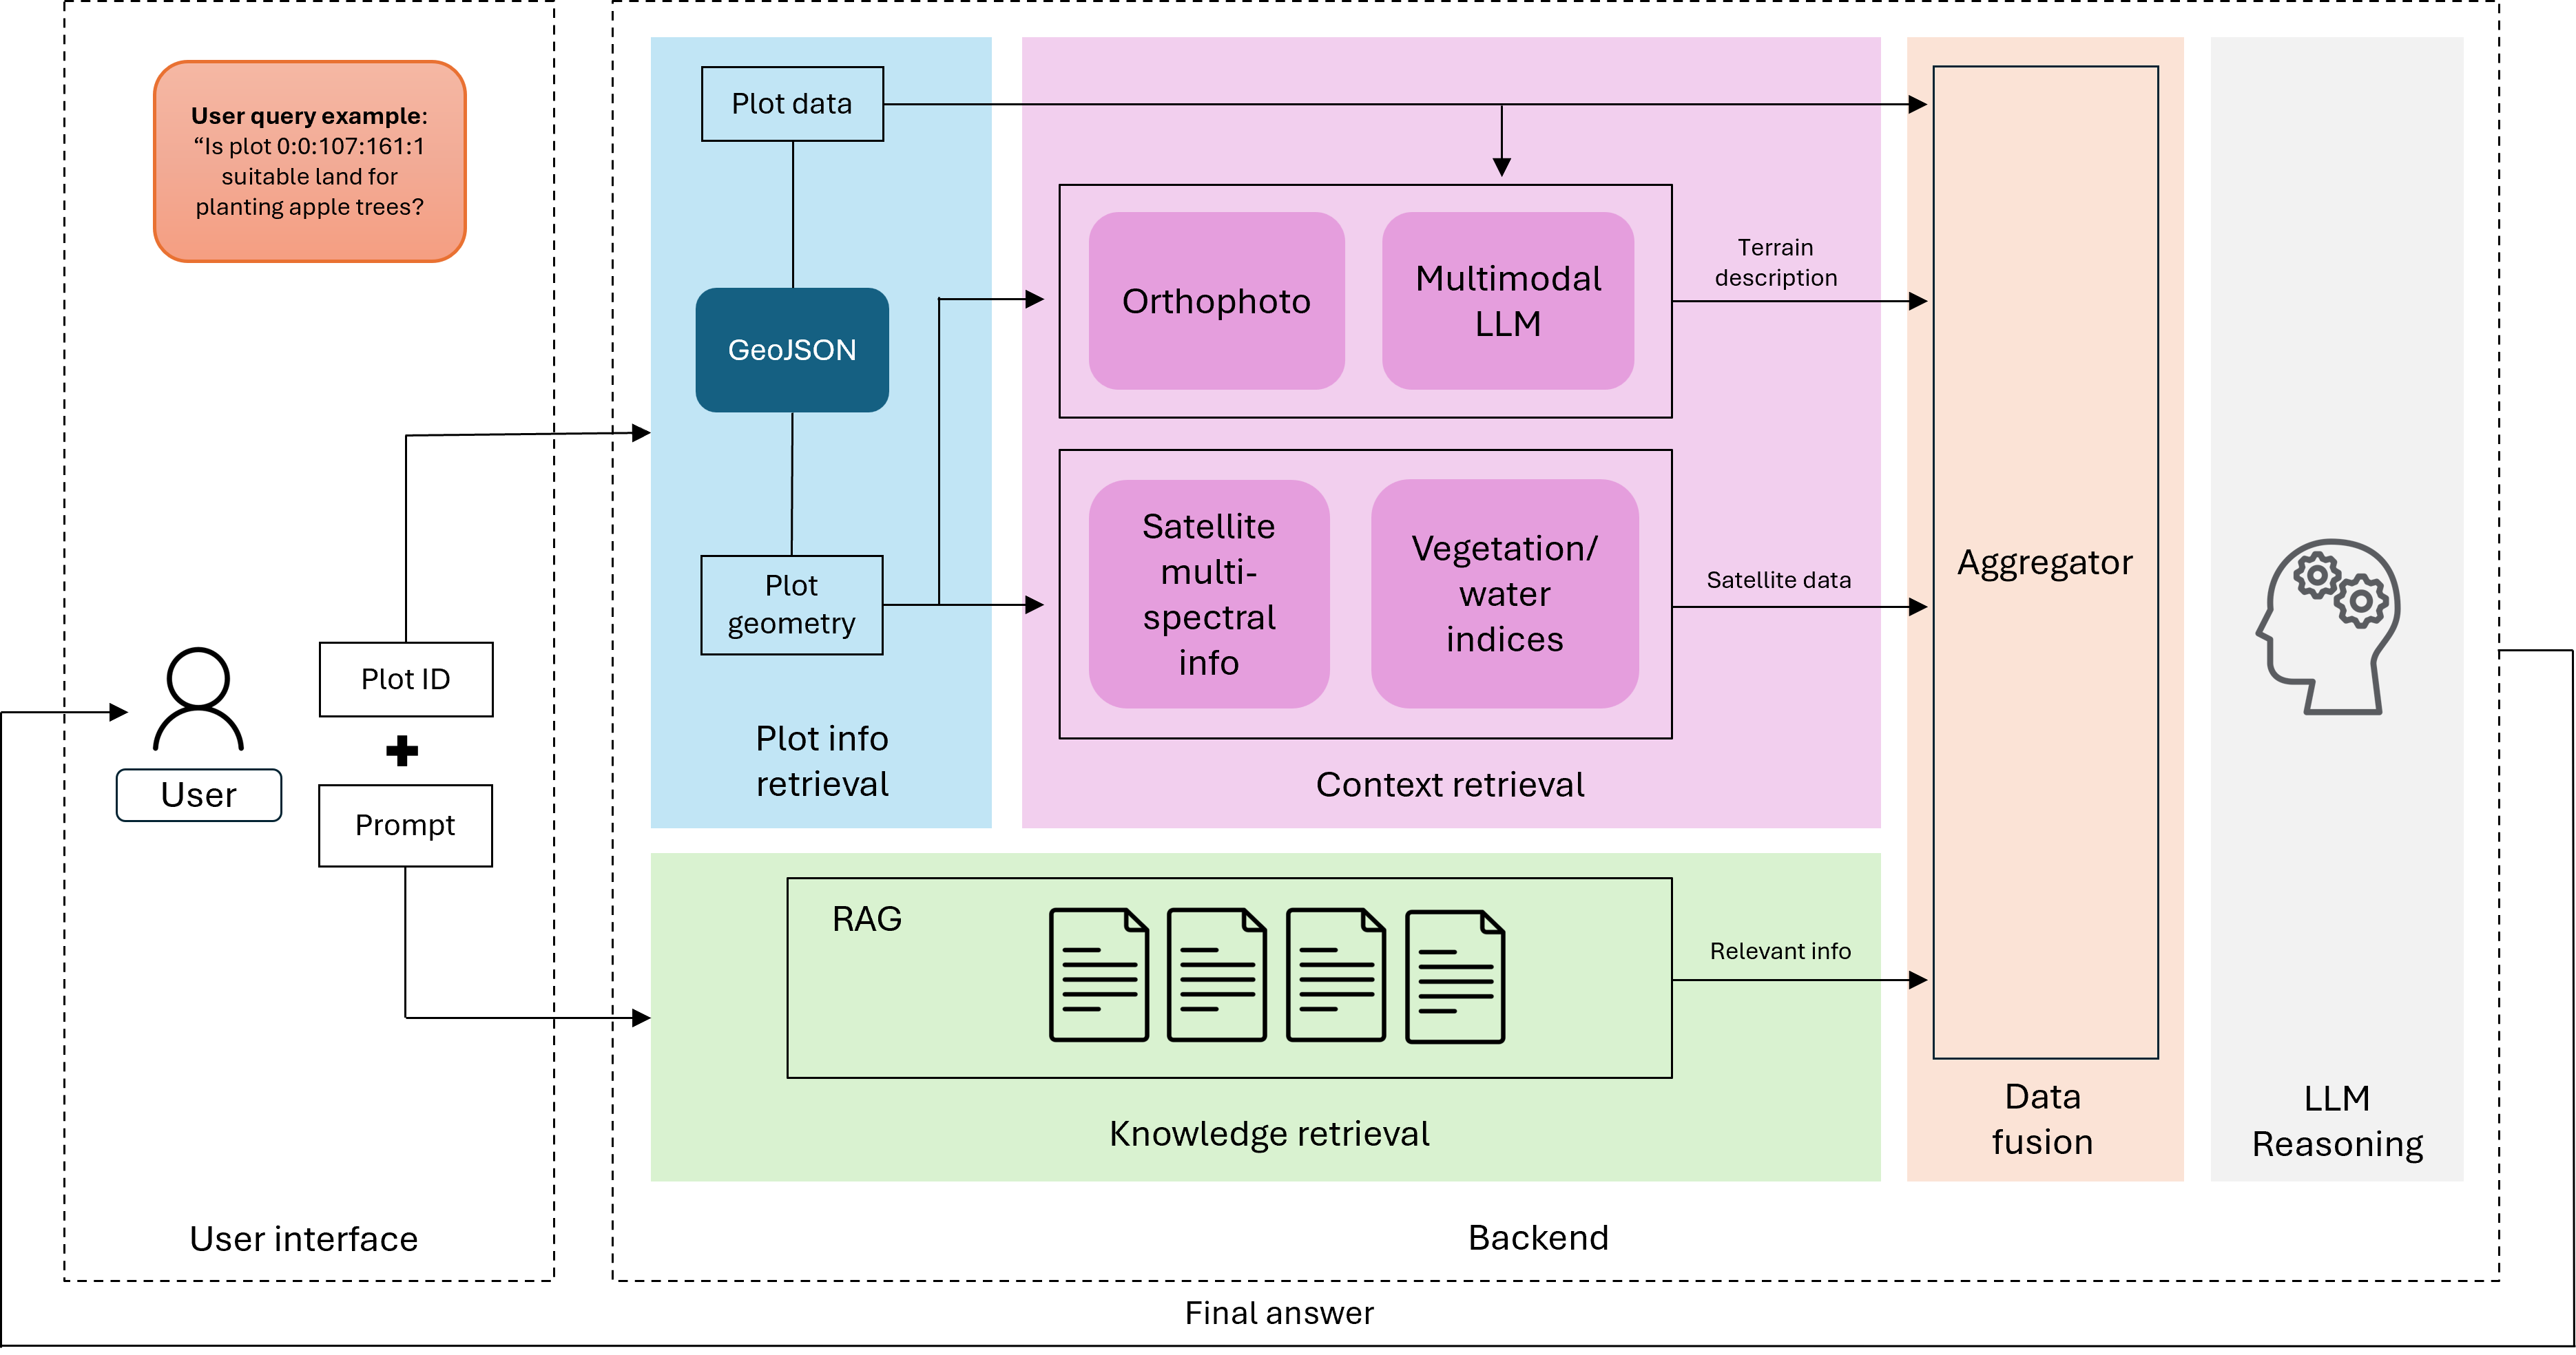
\includegraphics[width=\textwidth]{PIC/diagram.png}
	\caption{System architecture.}
	\label{fig:architecture}%
\end{figure*}

% \subsection{System overview}

% \textcolor{red}{copiado y opegado del otro paper: }

% The proposed system is designed to combine several in
% terconnected modules, which integrate heterogeneous data
% sources. The overall architecture, included in Fig. \ref{fig:architecture}, is composed of two main layers: user interface and backend processing, which includes the LLM reasoning. The aim of the data flow is to provide the final LLM with the most rich context regarding the area of interest (a specific parcel) in order for it
% to give the best possible answer to the user’s query.

% The backend consists of five different blocks, which con
% form a data stream from the user query to the final LLM, and
% then back to the user with the answer: (i) plot info retrieval,
% which is responsible for fetching, from the SIGPAC registry,
% both plot data-as slope, elevation, area, perimeter or land use
% , and the geo-referenced geometry. Once known the area of
% interest, the (ii) context retrieval block performs two parallel
% tasks, each leveraging different open-source data sources to
% enrich the context: (a) an ortophoto of the plot, obtained
% from aerial imagery, is processed through a multimodal LLM
% along with the plot data, generating a detailed description
% of the terrain. In addition, (b) satellite multispectral data,
% specifically from Sentinel-2 (Copernicus mission, European
% Spacial Agency) are retrieved. After spacial and temporal
% processing combining multiple spectral bands, an array of
% vegetation and water indices that reflect biophysical conditions
% of the land are obtained. In parallel, (iii) the system queries a
% document repository through a retrieval-augmented generation
% mechanism, which provides relevant textual knowledge such as
% agronomic guidelines, regulations, or best practices. All these
% multi-domain data are then fused through (iv) an aggregator,
% which converts all data to natural language, and prepares the
% information into an encapsulated prompt that provides the
% (v) final LLM with the overall context of the plot and the
% query. Several open-source models were evaluated, including
% Qwen3-32B, Llama-3.3-70B or Mistral-Small-3.2-24B, being
% Qwen the one chosen for the final implementation due to its
% superior performance. Regarding the LLMs framework, the
% model inference is managed with the inference engine vLLM
% [9], orchestrated through the liteLLM proxy [10], which ag
% glutinates all models in one port. Besides from the multimodal
% and final LLMs, there are also embeddings, reranker, and tool
% triage models working together. The infrasctructure runs in a
% 8x80GB cluster of NVIDIA GPUs.

\subsection{System Architecture and Overview}
The proposed system integrates heterogeneous geospatial, remote sensing, and agronomic domain knowledge into a unified data processing pipeline to ground the reasoning of a Large Language Model (LLM). As illustrated in Fig.~\ref{fig:architecture}, the architecture is structured into two primary layers: the \textit{User Interface} and the \textit{Backend Processing} pipeline. The core objective is to enrich the user's inquiry regarding a specific agricultural plot with multi-modal and biophysical context, enabling precise, evidence-based agronomic recommendations. The execution pipeline proceeds through five coordinated stages: (I) Plot Info Retrieval: The user provides a target plot identifier along with a natural language query. The system queries the geographic information system registry (SIGPAC) to retrieve plot-level attributes—including slope, elevation, surface area, perimeter, and registered land use—along with its georeferenced boundary geometry (encoded as GeoJSON). Hereafter, this piece of context is regarded as Plot Data. (II) Context Retrieval: Exploiting the extracted plot geometry, this module orchestrates two parallel multi-modal processing workflows: (II-a) Visual terrain analysis: High-resolution aerial imagery (orthophoto) covering the delineated plot is retrieved and processed by a Multimodal Large Language Model (MLLM) conditioned on the geometric and cadastral metadata, yielding a structured natural-language description of terrain topology, visible infrastructure, and surface patterns. (II-b) Biophysical state extraction: Multi-spectral imagery from the Sentinel-2 constellation (Copernicus, European Space Agency) is acquired. Following spatio-temporal filtering and band synthesis over the plot geometry, the pipeline computes a set of spectral vegetation and water indices, including NDVI and NDWI. (III) Knowledge Retrieval: In parallel with context generation, a Retrieval-Augmented Generation (RAG) subsystem queries a document repository created by the user. (IV) Data Fusion and Context Aggregation: The diverse data modalities—cadastral metadata, MLLM-derived terrain descriptions, remote sensing spectral indices, and retrieved textual context—are aligned and harmonized within an aggregator. This module serializes multi-source representations into a structured natural-language prompt context. (V) LLM Reasoning and Answer Generation: The synthesized prompt is fed to the central reasoning LLM, which integrates the holistic parcel profile to formulate the final recommendations delivered back to the user. For further details on the inference framework and technical hardware and software components, see \cite{juan_2025}. 

\subsection{Evaluation Framework}

The architectural characteristics of the proposed system dictate the requirements for its evaluation methodology. Crucially, this framework is not conceived merely as an \textit{ad-hoc} assessment for this specific tool, but rather as a reproducible and adaptable evaluation standard for any modular conversational agent relying on augmented external context. The primary challenge distinguishing this methodology from standard LLM benchmarks is the necessity to evaluate the actual utilization of geospatial context during response generation, going beyond mere response quality. An output that is factually correct but generic—or generated solely from the model's parametric memory—cannot be considered equivalent to a highly personalized recommendation grounded in the specific biophysical traits of a given terrain. Consequently, a comprehensive methodology combining multiple experimental phases, modular configurations, and tailored metrics has been designed. 

\subsubsection{Parcel Selection and Heterogeneity}

The study was carried out over a total of 15 target parcels, covering four distinct Land Use (LU) types: Fruit trees (FR), Pasture (PA), Unproductive (UN) and Forest (FO). The distribution of samples within Land Uses, as well as the volume of evaluation queries per parcel, is weighted according to the operational utility of the tool for each functional land use. 7 out of the 15 parcels belong to Fruit trees category, 4 are Pastures, and the remainer Unproductive and Forest land uses get 2 parcels each. Both the number of parcels per LU and the number of queries per parcel, are detailed in Table \ref{tab:num_queries_parcels}. \textcolor{red}{ Pendiente la parte de Fernando → Furthermore, the selected parcels exhibit a high degree of physical and geographical heterogeneity to stress-test the system under diverse conditions. This variance includes distinct topographies with slopes ranging from $0.5\%$ to $21.6\%$, varying altitudes, highly irregular geometric boundaries, and significant diversity in vegetative health, as captured by variable NDVI ranges. The spatial distribution and morphological characteristics of these parcels are illustrated in Fig. \ref{fig:parcel_mosaic}. Referencia a Fig. \ref{fig:map_qgis}.}

\begin{figure}[h!]
	\centering
	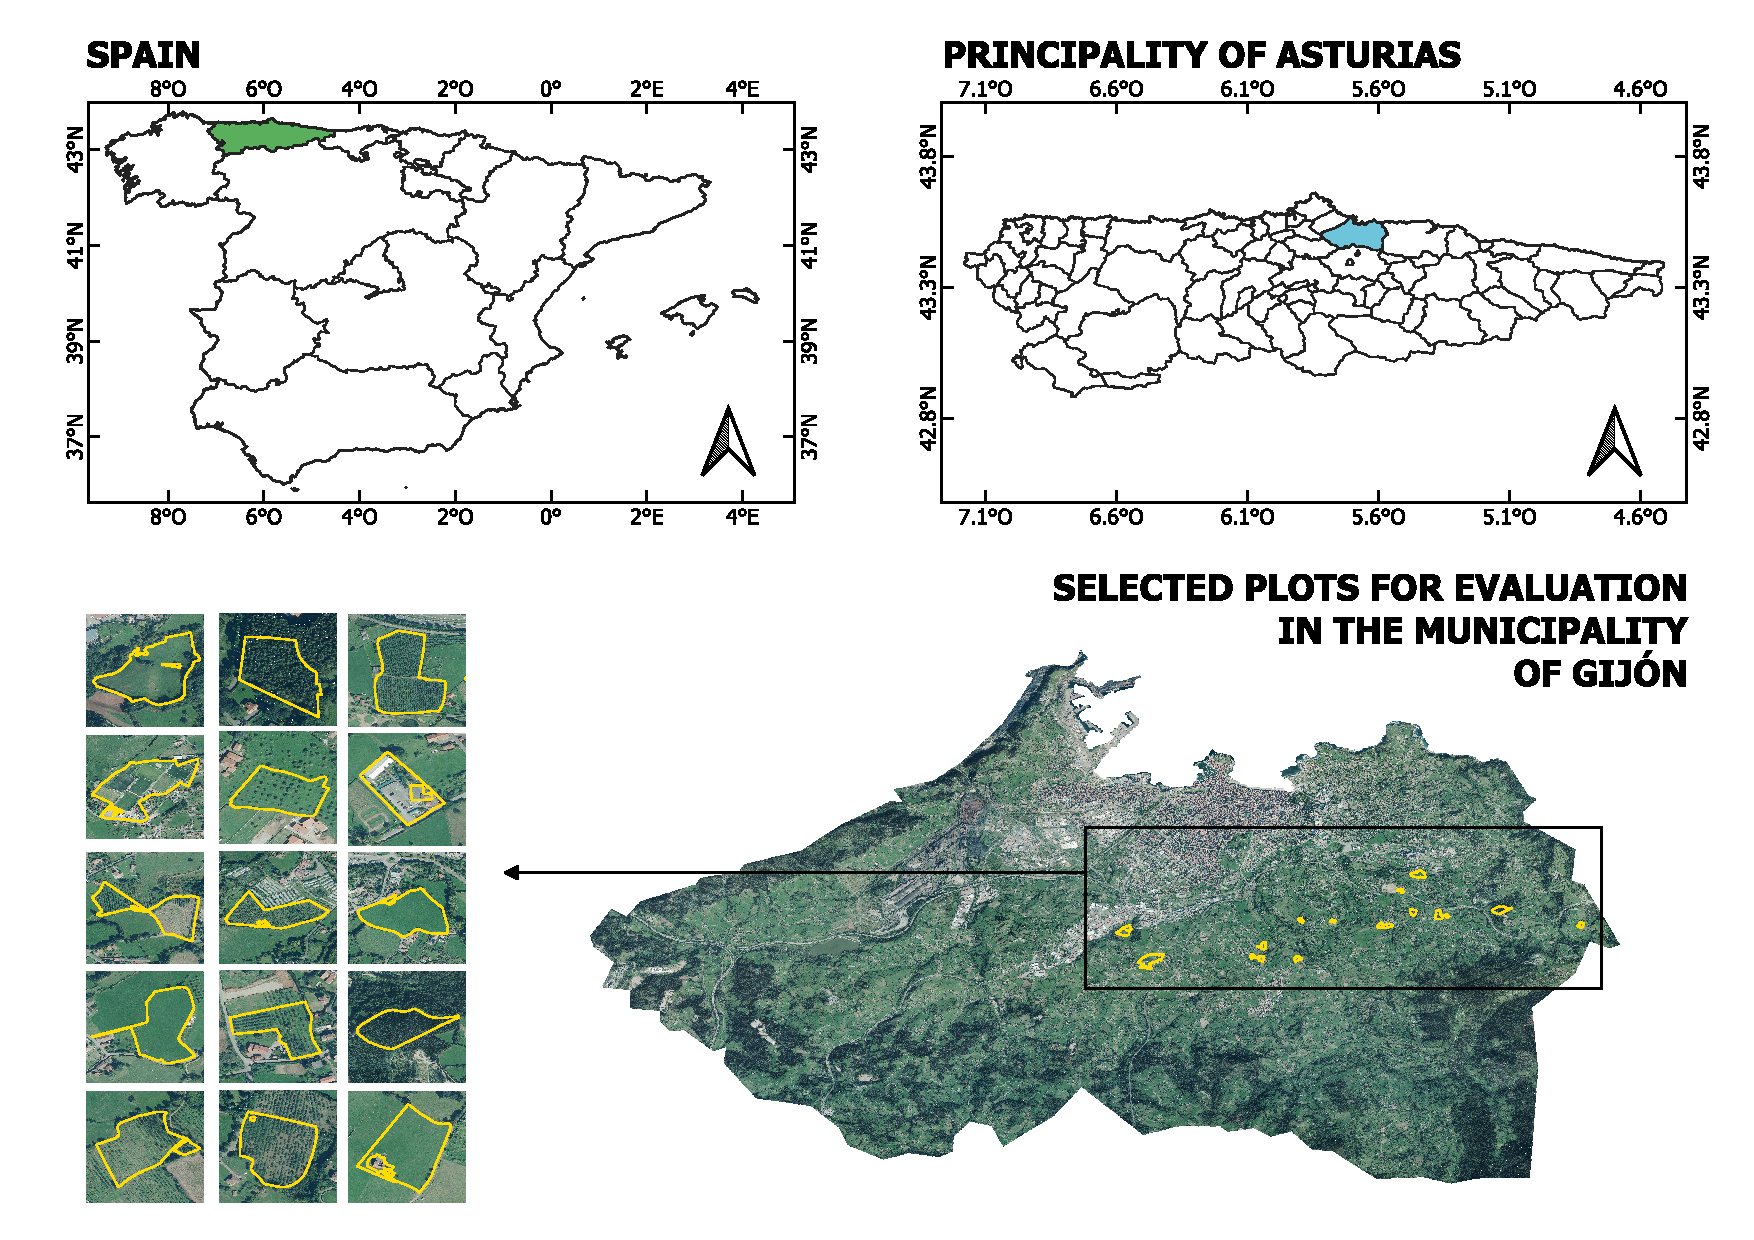
\includegraphics[width=\columnwidth]{PIC/Mapa_CEA_v4.pdf}
	\caption{The area of study in Gijón, Asturias. Location of the 15 selected parcels.}
	\label{fig:map_qgis}
\end{figure}

\subsubsection{Two-Stage Experimental Design}
The evaluation pipeline is structured into two main sequential phases to optimize operational resources while maintaining statistical robustness: an overall performance assessment and an ablation study. The first phase, named \textit{Broad Performance Assessment}, evaluates the system's holistic capability across diverse scenarios, using the full architecture. This stage does not represent a novel contribution, as it is similar to existing evaluation methods; rather, it provides an overall view of the quality of the responses in general terms, which is necessary before moving on to a more specific evaluation of the architecture modules. Table \ref{tab:num_queries_parcels} contians the number of evaluation queries, resulting in roughly 50$\%$ for each stage.

The second phase consists of an \textit{Ablation Study} intended to quantify the marginal contribution of each architectural component (Orthophoto, Satellite, and RAG modules, previously introduced in Fig. \ref{fig:architecture}). The concept of ablation study, originally rooted in medicine and biology to describe the surgical removal of tissue to determine its physiological function, has been adapted to the field of artificial intelligence and proved as a valid paradigm to uncover individual contributions by isolating components. In \cite{meyes_ablation_2020}, they use the concept of ablation for finding redundancies in the representations of Artifitial Neural Networks. In this work, we extend this analytical framework to evaluate our proposed modular methodology by progressively isolating and bypassing individual modules. For this porpuse, a full factorial design of experiments was executed to set up the configurations, which are combinations of the modules, summarized in Fig. \ref{fig:ablation_modules}. By systematically enabling and disabling these three external context modules, $2^3 = 8$ configurations were generated, plus a Zero-Shot baseline, where the LLM reasons without any external parcel context, for a total of 9 configurations, as detailed in Table \ref{tab:ablation_configs}. For this phase, a representative subset of one parcel per LU category was selected, and 2 specific queries were executed across all 9 configurations, yielding 72 additional evaluations (\ref{tab:num_queries_parcels}).

\begin{figure}[h!]
	\centering
	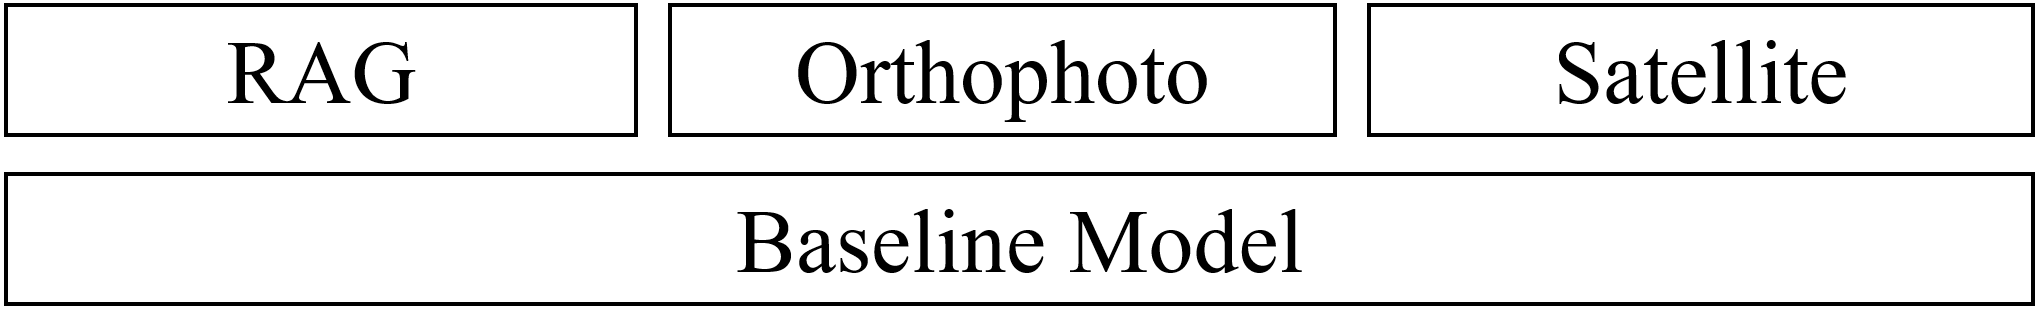
\includegraphics[width=\columnwidth]{PIC/ablation_modules.png}
	\caption{Ablation modules.}
	\label{fig:ablation_modules}
\end{figure}

\begin{table*}[t!]
	\caption{Configuraciones modulares del estudio de ablación. PD means Plot Data. Active tool is always enabled because it is responsible for identifying parcel IDs as so. }
	\label{tab:ablation_configs}
	\begin{tabular}{p{0.28\textwidth}
			p{0.07\textwidth}
			p{0.07\textwidth}
			p{0.07\textwidth}
			p{0.08\textwidth}
			p{0.17\textwidth}
			p{0.09\textwidth}
		}
		\hline
		\textbf{Modules} & \textbf{RAG} & \textbf{ORTHO} & \textbf{SAT} & \textbf{PD} & \textbf{Active Tool} & \textbf{Code} \\
		\hline
		Baseline         & 0            & 0              & 0            & 1           & 1                    & 0             \\
		B + SAT          & 0            & 0              & 1            & 1           & 1                    & 1             \\
		B + ORTHO        & 0            & 1              & 0            & 1           & 1                    & 2             \\
		B + ORTHO + SAT  & 0            & 1              & 1            & 1           & 1                    & 3             \\
		B + RAG          & 1            & 0              & 0            & 1           & 1                    & 4             \\
		B + RAG + SAT    & 1            & 0              & 1            & 1           & 1                    & 5             \\
		B + RAG + ORTHO  & 1            & 1              & 0            & 1           & 1                    & 6             \\
		Complete         & 1            & 1              & 1            & 1           & 1                    & 7             \\
		ZERO SHOT        & 0            & 0              & 0            & 0           & 1                    & ZS            \\
		\hline
	\end{tabular}
\end{table*}

Ultimately, the combined phases produced a comprehensive evaluation dataset of 143. The full dataset containing queries, retrieved contexts, and generated responses is publicly available (see Appendix A). \textcolor{red}{Ref a Zenodo}

\subsubsection{Panel of judges}

A simplified approach to response evaluation, as utilized in our previous work, relies exclusively on the LLM-as-a-judge framework. This paradigm offers distinct advantages in terms of execution speed and scalability, allowing for the rapid assessment of large datasets without the bottlenecks associated with human review. Conversely, assembling a panel of human evaluators requires substantial planning, timeframes, and financial resources. However, human evaluation remains indispensable, as it fundamentally reduces the leniency bias frequently exhibited by LLM evaluators (\cite{gu_survey_2026}) and provides a significantly higher degree of reliability when assessing nuanced, domain-specific reasoning. To effectively navigate this trade-off between scalability and qualitative rigor, we designed a hybrid, human-in-the-loop evaluation strategy. By merging human and machine critical judgement, this methodology not only optimizes resource allocation but also systematically mitigates the mono-dimensional biases inherent to using either approach in isolation. 

Consequently, the definitive panel of judges comprises four distinct entities: two human evaluators and two LLM-based evaluators. To ensure both technical depth and practical accessibility, the human contingent is divided into two distinct roles, a domain expert (holding a PhD in Biology), regarded hereafter as "Human Expert (H$\_$E)" that provides rigorous scientific scrutiny; and a control evaluator, regarded as "Human Control (H$\_$C), representing the end-user perspective in terms of clarity and usability for non-academic audience. For the LLM side, we integrated two diverse language models with comparable computational footprints into the panel: a propietary model, Gemini 3.1 Flash Lite, and an open-source model, Qwen3.5-397B-A17B-Instruct.

\subsection{Multidimensional metrics}

The quality of the generated responses is quantified using a multidimensional 5-point Likert scale encompassing five distinct criteria (see Table \ref{tab:evaluation_metrics}). Four of these metrics—Correctness, Completeness, Relevance, and Utility—evaluate the intrinsic quality of the response and can be assessed without access to the retrieved context. Conversely, the \textit{Grounding} metric strictly requires contextual reference; it is specifically designed to measure the degree to which the formulated response is faithfully derived from the injected multi-domain data rather than the model's pre-existing generalized knowledge. 

\begin{table}[h!]
	\caption{Multidimensional evaluation metrics framework. Note: The \textit{Grounding} metric measures the degree to which responses are derived from the obtained context, rather than generic knowledge, making it the only metric requiring context for evaluation.}
	\label{tab:evaluation_metrics}
	\begin{tabular}{
			>{\raggedright\arraybackslash}p{0.6\columnwidth}
			>{\raggedright\arraybackslash}p{0.3\columnwidth}
		}
		\hline
		\textbf{Metric} & \textbf{Type}   \\
		\hline
		Correctness     & Without Context \\
		Completeness    & Without Context \\
		Relevance       & Without Context \\
		Utility         & Without Context \\
		\hline
		Grounding       & With Context    \\
		\hline
	\end{tabular}
\end{table}

\textcolor{red}{Internal Knowledge over-reliance → sesgo de conocimiento interno}

\begin{figure*}[t]
	\centering{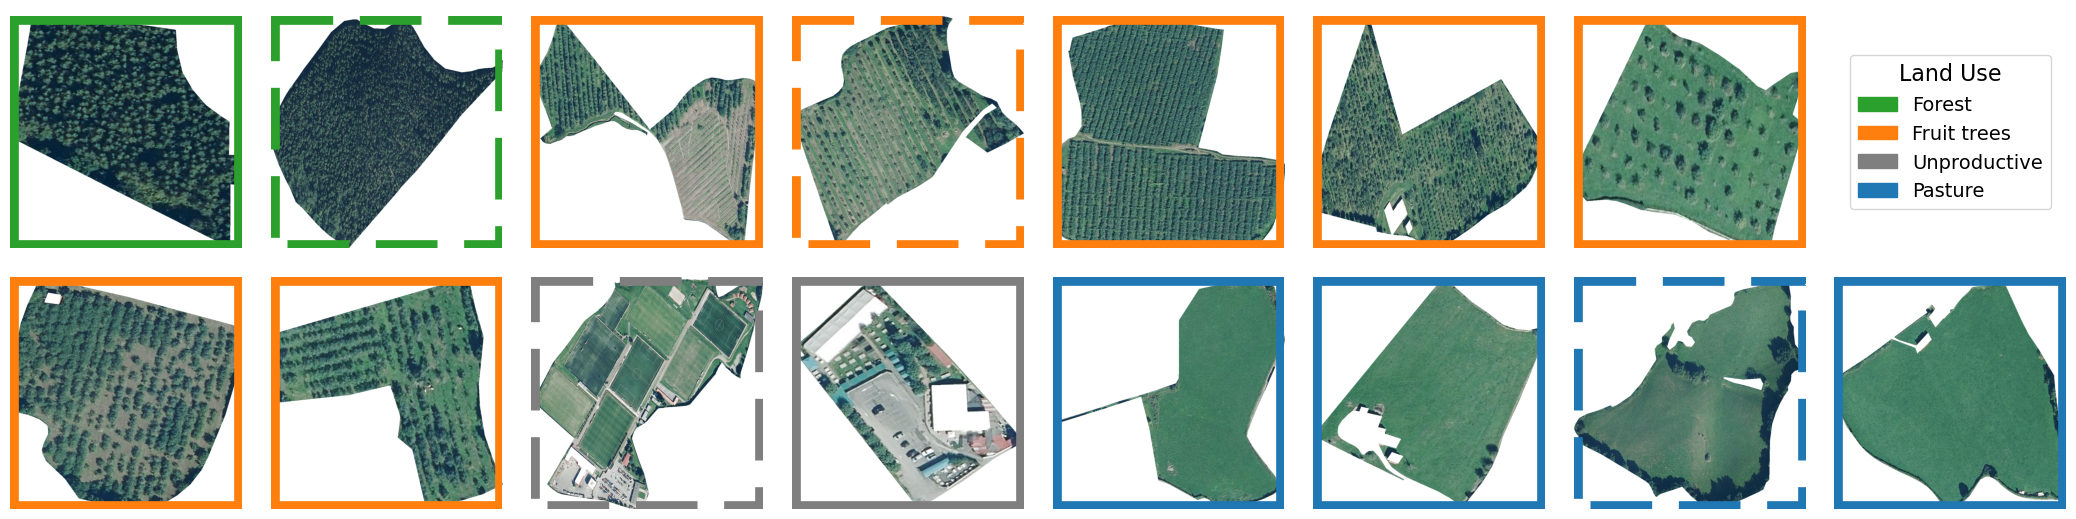
\includegraphics[width=\textwidth]{PIC/mosaic_2x8_white_bg_ablation.png}}
	\caption{Selection of parcels for tool evaluation, grouped by Land Use. The number of parcels per LU depends on their functional utility in agriculture. Dashed borders correspond to parcels used in ablation study.}
	\label{fig:parcel_mosaic}
\end{figure*}

% \begin{table}[h!]
% 	\caption{Distribution of parcels by Land Use (LU) type}
% 	\label{tab:land_use}
% 	\begin{tabular}{p{0.5\columnwidth}
%         >{\raggedright\arraybackslash}p{0.40\columnwidth}
% 		>{\raggedright\arraybackslash}p{0.40\columnwidth}
% 		}
% 		\hline
% 		\textbf{Land Use} & \textbf{Num. of parcels} & \textbf{Queries per parcel} & \textbf{Total queries} \\
% 		\hline
% 		Fruit Trees (FR)  & 7                          \\
% 		Pasture (PA)      & 4                          \\
% 		Unproductive (UN) & 2                          \\
% 		Forest (FO)       & 2                          \\
% 		\hline
% 	\end{tabular}
% \end{table}

\begin{itemize}
	\item \textbf{Configurations:} 8 modular combinations + 1 Zero-Shot baseline (the LLM without parcel context) = 9 total configurations, listed in \ref{tab:ablation_configs}.
	\item \textbf{Sample subset:} 1 representative parcel per Land Use category.
	\item \textbf{Query volume:} 2 specific queries per parcel across the 9 configurations $= \mathbf{72 \text{queries}}$.
\end{itemize}

\subsection{Evaluation Volume Summary}

\begin{table*}[t]
\centering
\caption{Distribution of parcels, queries, and configurations across methodology stages for each land use category.}
\label{tab:num_queries_parcels}
% Reducimos ligeramente el padding entre columnas para 9 columnas
\setlength{\tabcolsep}{3.5pt} 

% Fijamos el ancho total a 0.8\textwidth
\begin{tabularx}{\textwidth}{l *{8}{Y}}
\toprule
\multirow{2}{*}{\textbf{Land Use}} 
  & \multicolumn{3}{c}{\textbf{Broad}} 
  & \multicolumn{4}{c}{\textbf{Ablation}} 
  & \multirow{2}{*}{\textbf{Total}} \\
\cmidrule(lr){2-4} \cmidrule(lr){5-8}
  & \textbf{No. parcels} & \textbf{Queries/ parcel} & \textbf{No. queries} 
  & \textbf{No. parcels} & \textbf{Queries/ parcel} & \textbf{No. configs} & \textbf{No. queries} 
  & \\
\midrule
Fruit trees (FR)   & 7 & 5 & 35 & 1 & 2 & 9 & 18 & -- \\
Pasture (PA)       & 4 & 5 & 20 & 1 & 2 & 9 & 18 & -- \\
Forest (FO)        & 2 & 4 &  8 & 1 & 2 & 9 & 18 & -- \\
Unproductive (UN)  & 2 & 4 &  8 & 1 & 2 & 9 & 18 & -- \\
\midrule
\textbf{Total}     &   &   & \textbf{71} &   &   &   & \textbf{72} & \textbf{143} \\
\bottomrule
\end{tabularx}
\end{table*}


% \begin{table}[h!]
% 	\caption{Summary of total query volume in the evaluation.}
% 	\label{tab:evaluation_summary}
% 	\begin{tabular}{
% 			p{0.34\columnwidth}
% 			p{0.22\columnwidth}
% 			>{\raggedleft\arraybackslash}p{0.3\columnwidth}
% 		}
% 		\hline
% 		\textbf{Evaluation Phase} & \textbf{Methodology} & \textbf{Num. of queries} \\
% 		\hline
% 		Broad Assessment          & Sequential           & 71                    \\
% 		Ablation Study            & Simultaneous         & 72                    \\
% 		\hline
% 		\textbf{Total}            &                      & \textbf{143}          \\
% 		\hline
% 	\end{tabular}
% \end{table}

\begin{figure*}[t!]
	\centering{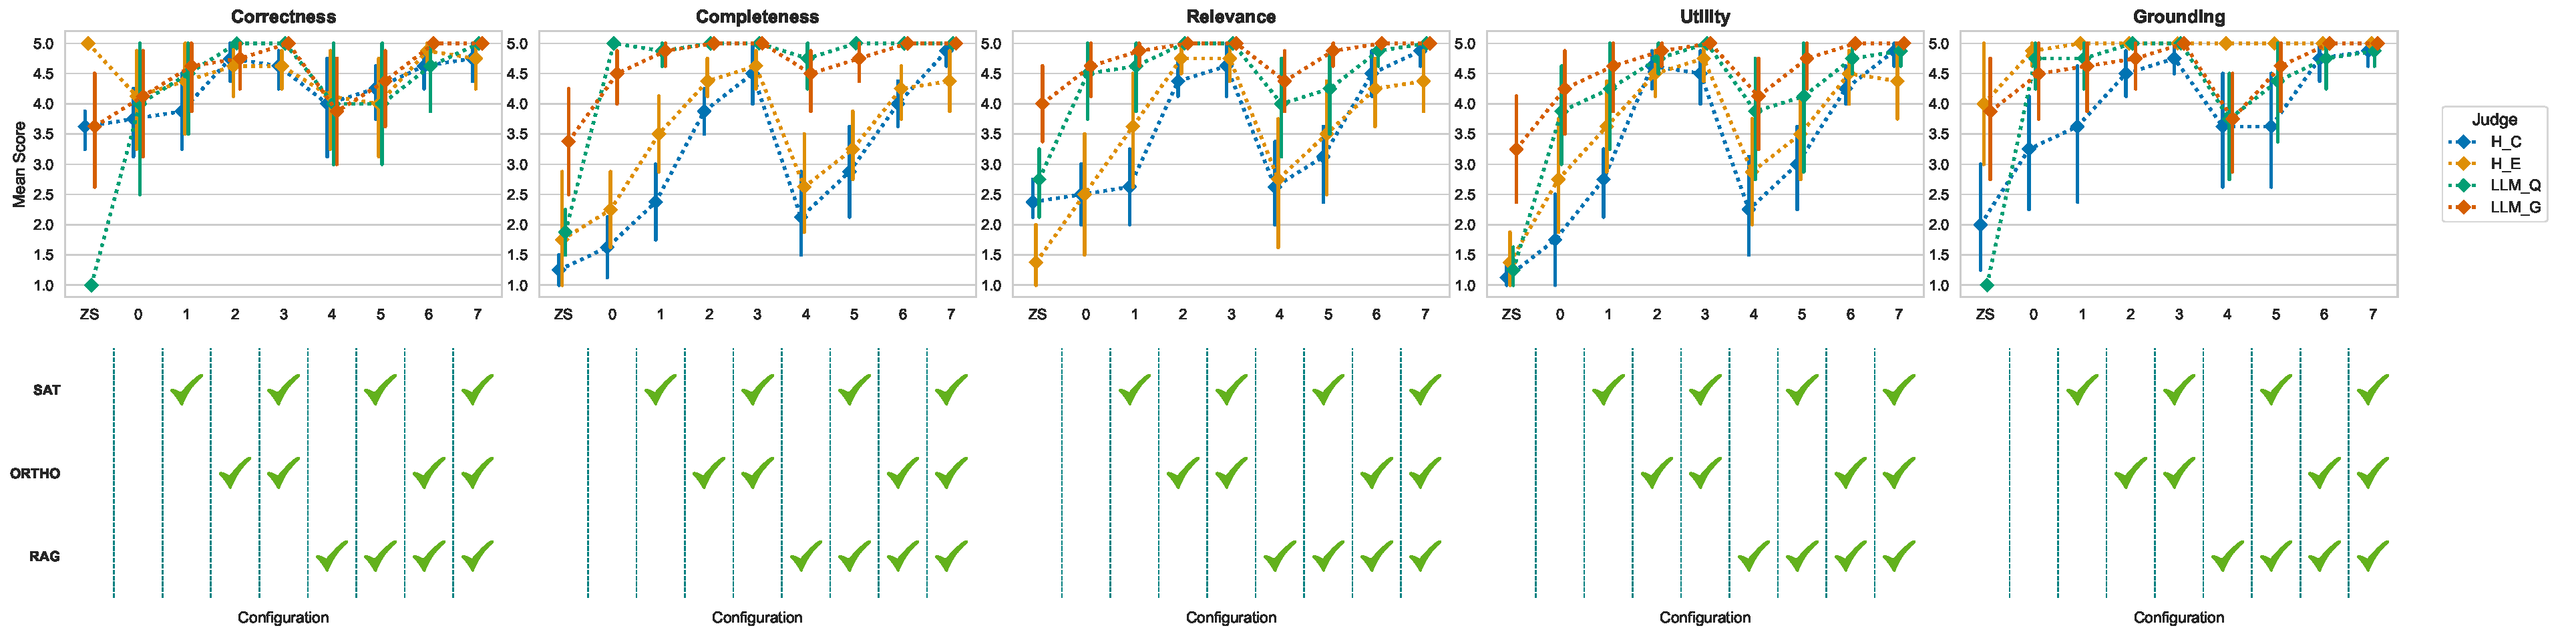
\includegraphics[width=\textwidth]{PIC/scores_configurations_tick.pdf}}
	\caption{Preliminary evaluation results from the \textit{Ablation Study} phase for the 4 evaluators and 5 metrics grouped by configuration. Differences can be observed based on active modules.}
	\label{fig:results}
\end{figure*}



\subsection{Preliminary Results and Discussion}

// TODO comentar sobre suficiente y necesario

This section presents some preliminary evaluation results. It should be noted that the graphs included here are only an initial overview that sheds light on the system evaluation; more advanced statistical analyses are reserved for a future scientific publication. First, \ref{fig:results} contains the average scores of each of the 4 evaluators across the 5 metrics, grouped by configuration. From this graph, numerous observations can be made, with the most notable being those related to evaluator correlation, and especially regarding the marginal contributions of the modules. Recalling \ref{tab:ablation_configs}, we see that configurations 2 and 3, as well as 6 and 7, include the orthophoto module; and in all metrics, a higher average score is observed in these cases, allowing us to deduce that the marginal contribution of the orthophoto module is significant.

\begin{table}[h!]
    \caption{.}
    \label{tab:bars}
    \begin{tabular}{
        >{\raggedright\arraybackslash}p{\dimexpr0.28\columnwidth-2\tabcolsep\relax}
        *{4}{>{\centering\arraybackslash}p{\dimexpr0.18\columnwidth-2\tabcolsep\relax}}
        }
        \hline
        \textbf{Metric} & \textbf{H\_C} & \textbf{H\_E} & \textbf{LLM\_Q} & \textbf{LLM\_G} \\
        \hline
        Correctness  & 4.690 & 4.704 & 4.817 & 4.746 \\
        Completeness & 4.803 & 4.817 & 4.944 & 4.958 \\
        Relevance    & 4.549 & 4.817 & 4.831 & 4.930 \\
        Utility      & 4.704 & 4.761 & 4.859 & 4.944 \\
        Grounding    & 4.606 & 4.901 & 4.296 & 4.549 \\
        \hline
    \end{tabular}
\end{table}

% \begin{figure}[h!]
% 	\centering
% 	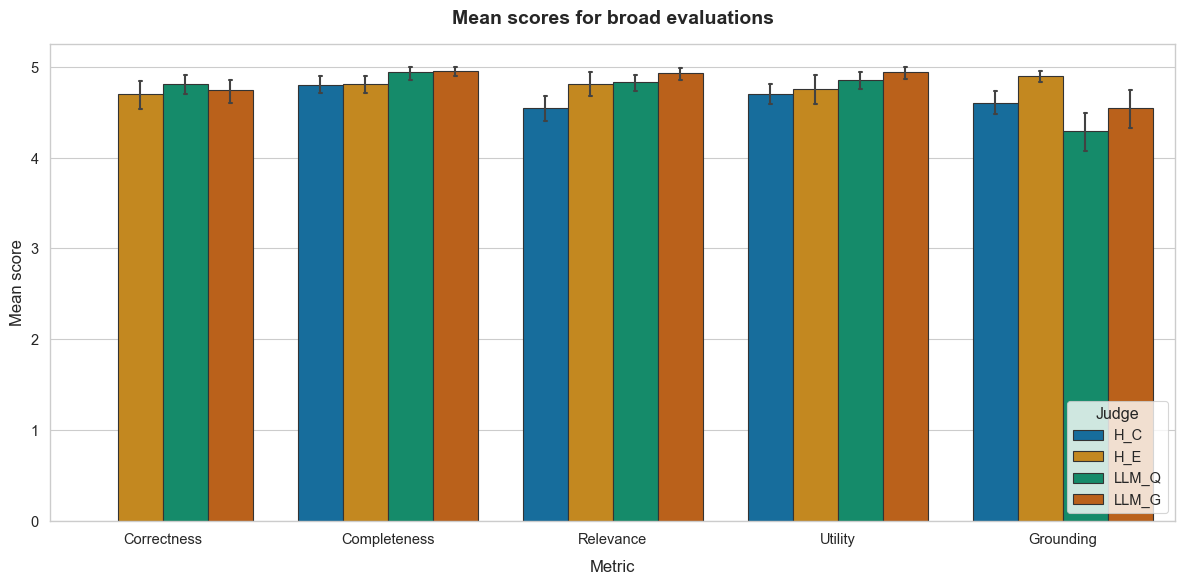
\includegraphics[width=\columnwidth]{PIC/broad_bars.png}
% 	\caption{Average values for the 4 evaluators and 5 metrics in the \textit{Broad} phase (complete system).}
% 	\label{fig:broad}
% \end{figure}

\begin{figure*}[h!]
	\centering
	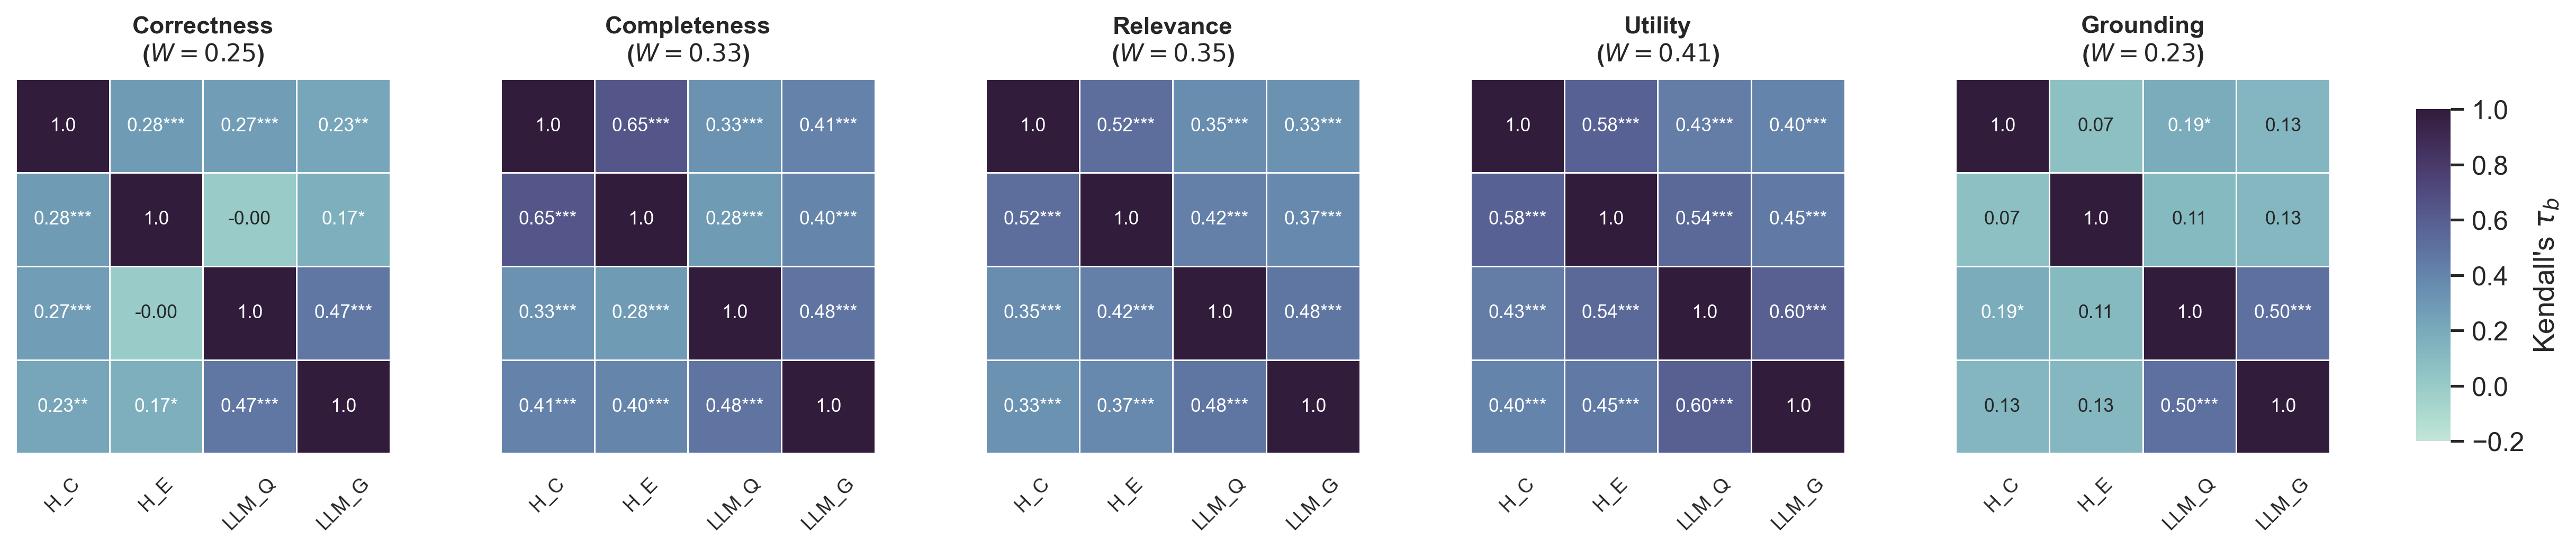
\includegraphics[width=\textwidth]{PIC/consensus.png}
	\caption{}
	\label{fig:consensus}
\end{figure*}

Similarly, the trend across all metrics is ascending along the x-axis (values are lower in left-side configurations), showing how, for example, system utility in the \textit{Zero Shot} configuration is below 1/5 for most evaluators. Since this configuration corresponds to a standard LLM model without context augmentation, and with configurations progressively ordered by active modules, it can be concluded that \textbf{responses, as expected, improve as more geospatial terrain information is added.} This result consequently verifies the initial hypothesis and validates the proposed architecture.

More generally, \ref{fig:broad} represents the average metric values from the \textit{Broad} stage evaluations, i.e., the complete system. For all evaluators, the resulting metrics average values very close to 5/5, implying that the system has responded with a high degree of success to the evaluated queries. These preliminary results serve as evidence that the proposed system is capable of generating high-quality, complete, useful, and generally successful responses in the broad sense.


Shapley Values

\begin{equation}
	\phi_i(v) = \sum_{S \subseteq N \setminus \{i\}} \frac{|S|!(|N| - |S| - 1)!}{|N|!} \big(v(S \cup \{i\}) - v(S)\big)
\end{equation}

$N$ is the set of all players: 
$N = \{M_{S}, M_{O}, M_{R}\}$ and 
$S$ is any subset or \textit{coalition}.

\begin{equation}
    \begin{split}
        \phi_S(v) = {} & \frac{1}{3} \big[ v(\{M_S\}) - v(\varnothing) \big]              \\
                    & + \frac{1}{6} \big[ v(\{M_S, M_O\}) - v(\{M_O\}) \big]           \\
                    & + \frac{1}{6} \big[ v(\{M_S, M_R\}) - v(\{M_R\}) \big]           \\
                    & + \frac{1}{3} \big[ v(\{M_S, M_O, M_R\}) - v(\{M_O, M_R\}) \big]
    \end{split}
\end{equation}

\begin{equation}
    \begin{split}
        \phi_O(v) = {} & \frac{1}{3}[v(\{M_O\})-v(\varnothing)]           \\
                    & +\frac{1}{6}[v(\{M_S, M_O\})-v(\{M_S\})]         \\
                    & +\frac{1}{6}[v(\{M_O, M_R\})-v(\{M_R\})]         \\
                    & +\frac{1}{3}[v(\{M_S, M_O,M_R\})-v(\{M_S,M_R\})]
    \end{split}
\end{equation}

\begin{equation}
    \begin{split}
        \phi_R(v) = {} & \frac{1}{3}[v(\{M_R\})-v(\varnothing)]           \\
                    & +\frac{1}{6}[v(\{M_S, M_R\})-v(\{M_S\})]         \\
                    & +\frac{1}{6}[v(\{M_O, M_R\})-v(\{M_O\})]         \\
                    & +\frac{1}{3}[v(\{M_S, M_O,M_R\})-v(\{M_S,M_O\})]
    \end{split}
\end{equation}

\begin{equation}
    \begin{split}
        \phi_S(v) = {} & \frac{1}{3}[v(C_1)-v(C_0)]+\frac{1}{6}[v(C_3)-v(C_2)]  \\
                    & +\frac{1}{6}[v(C_5)-v(C_4)]+\frac{1}{3}[v(C_7)-v(C_6)]
    \end{split}
\end{equation}

\begin{equation}
    \begin{split}
        \phi_O(v) = {} & \frac{1}{3}[v(C_2)-v(C_0)]+\frac{1}{6}[v(C_3)-v(C_1)]  \\
                    & +\frac{1}{6}[v(C_6)-v(C_4)]+\frac{1}{3}[v(C_7)-v(C_5)]
    \end{split}
\end{equation}

\begin{equation}
    \begin{split}
        \phi_R(v) = {} & \frac{1}{3}[v(C_4)-v(C_0)]+\frac{1}{6}[v(C_5)-v(C_1)]  \\
                    & +\frac{1}{6}[v(C_6)-v(C_2)]+\frac{1}{3}[v(C_7)-v(C_3)]
    \end{split}
\end{equation}

\begin{figure*}[t!]
	\centering{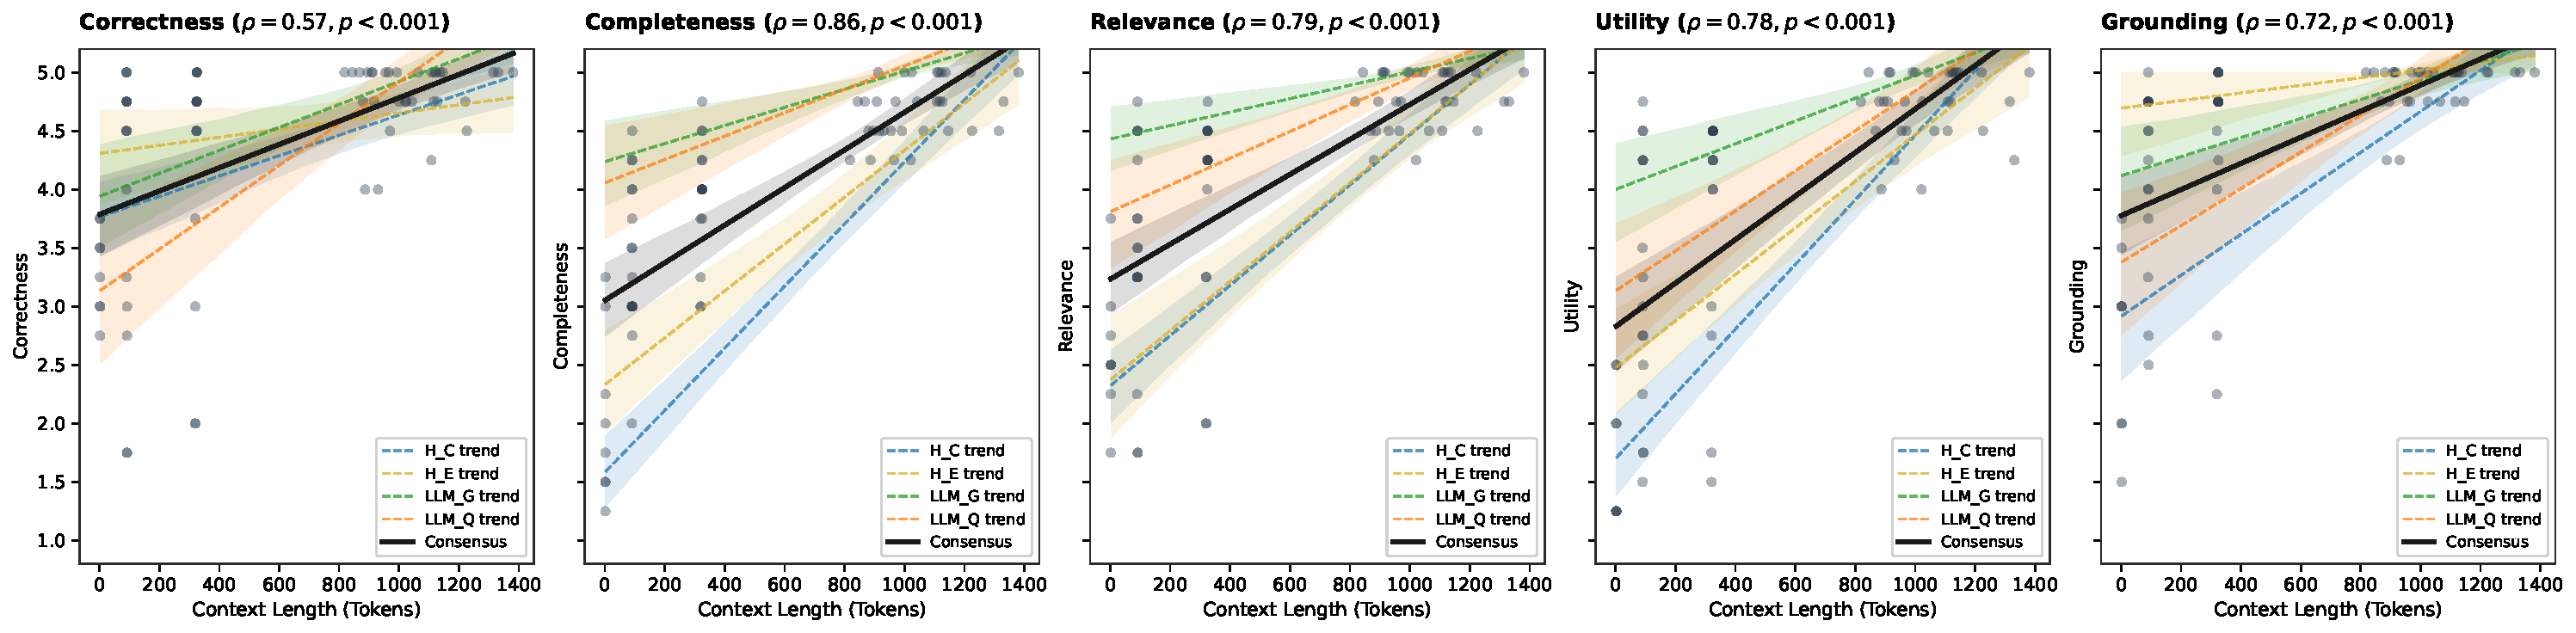
\includegraphics[width=\textwidth]{PIC/tokens_metrics.pdf}}
	\caption{}
	\label{fig:tokens_metrics}
\end{figure*}


\begin{figure*}[t]
	\centering{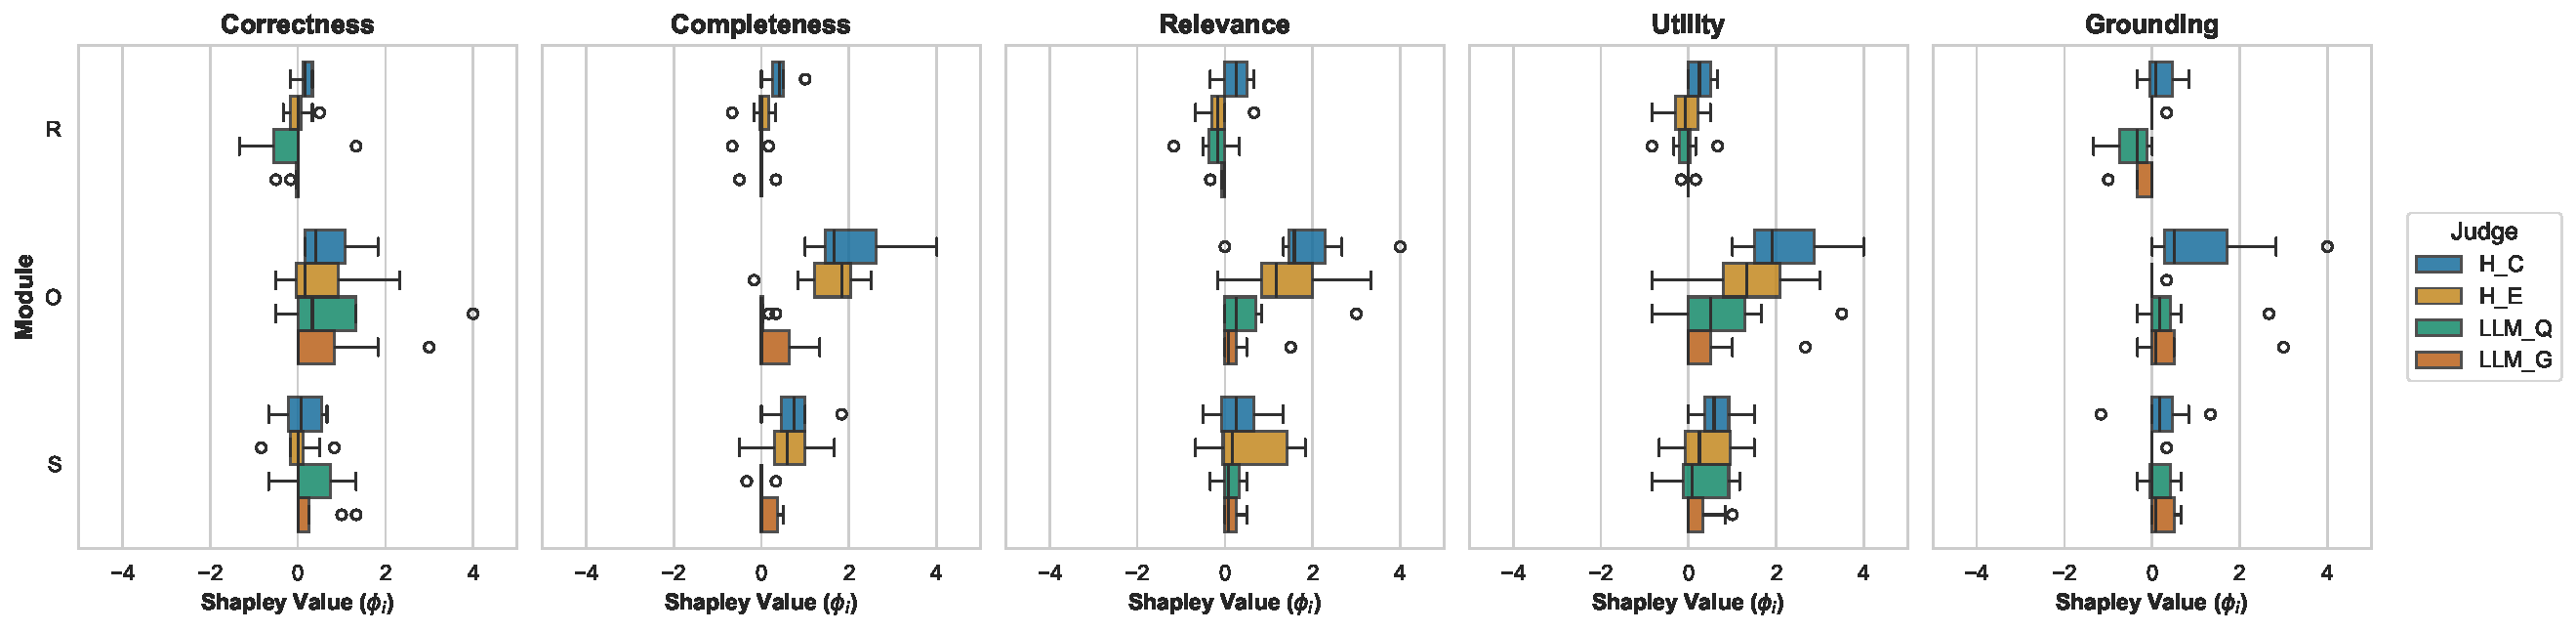
\includegraphics[width=\textwidth]{PIC/shapley_boxplots_horizontales.pdf}}
	\caption{}
	\label{fig:shapleys}
\end{figure*}

\textcolor{red}{Meter gráficas solo con valores del promedio de los 4 jueces para no crear ruido visual}

\section{Results and Discussion}

% \begin{figure}[t]
% 	\centering{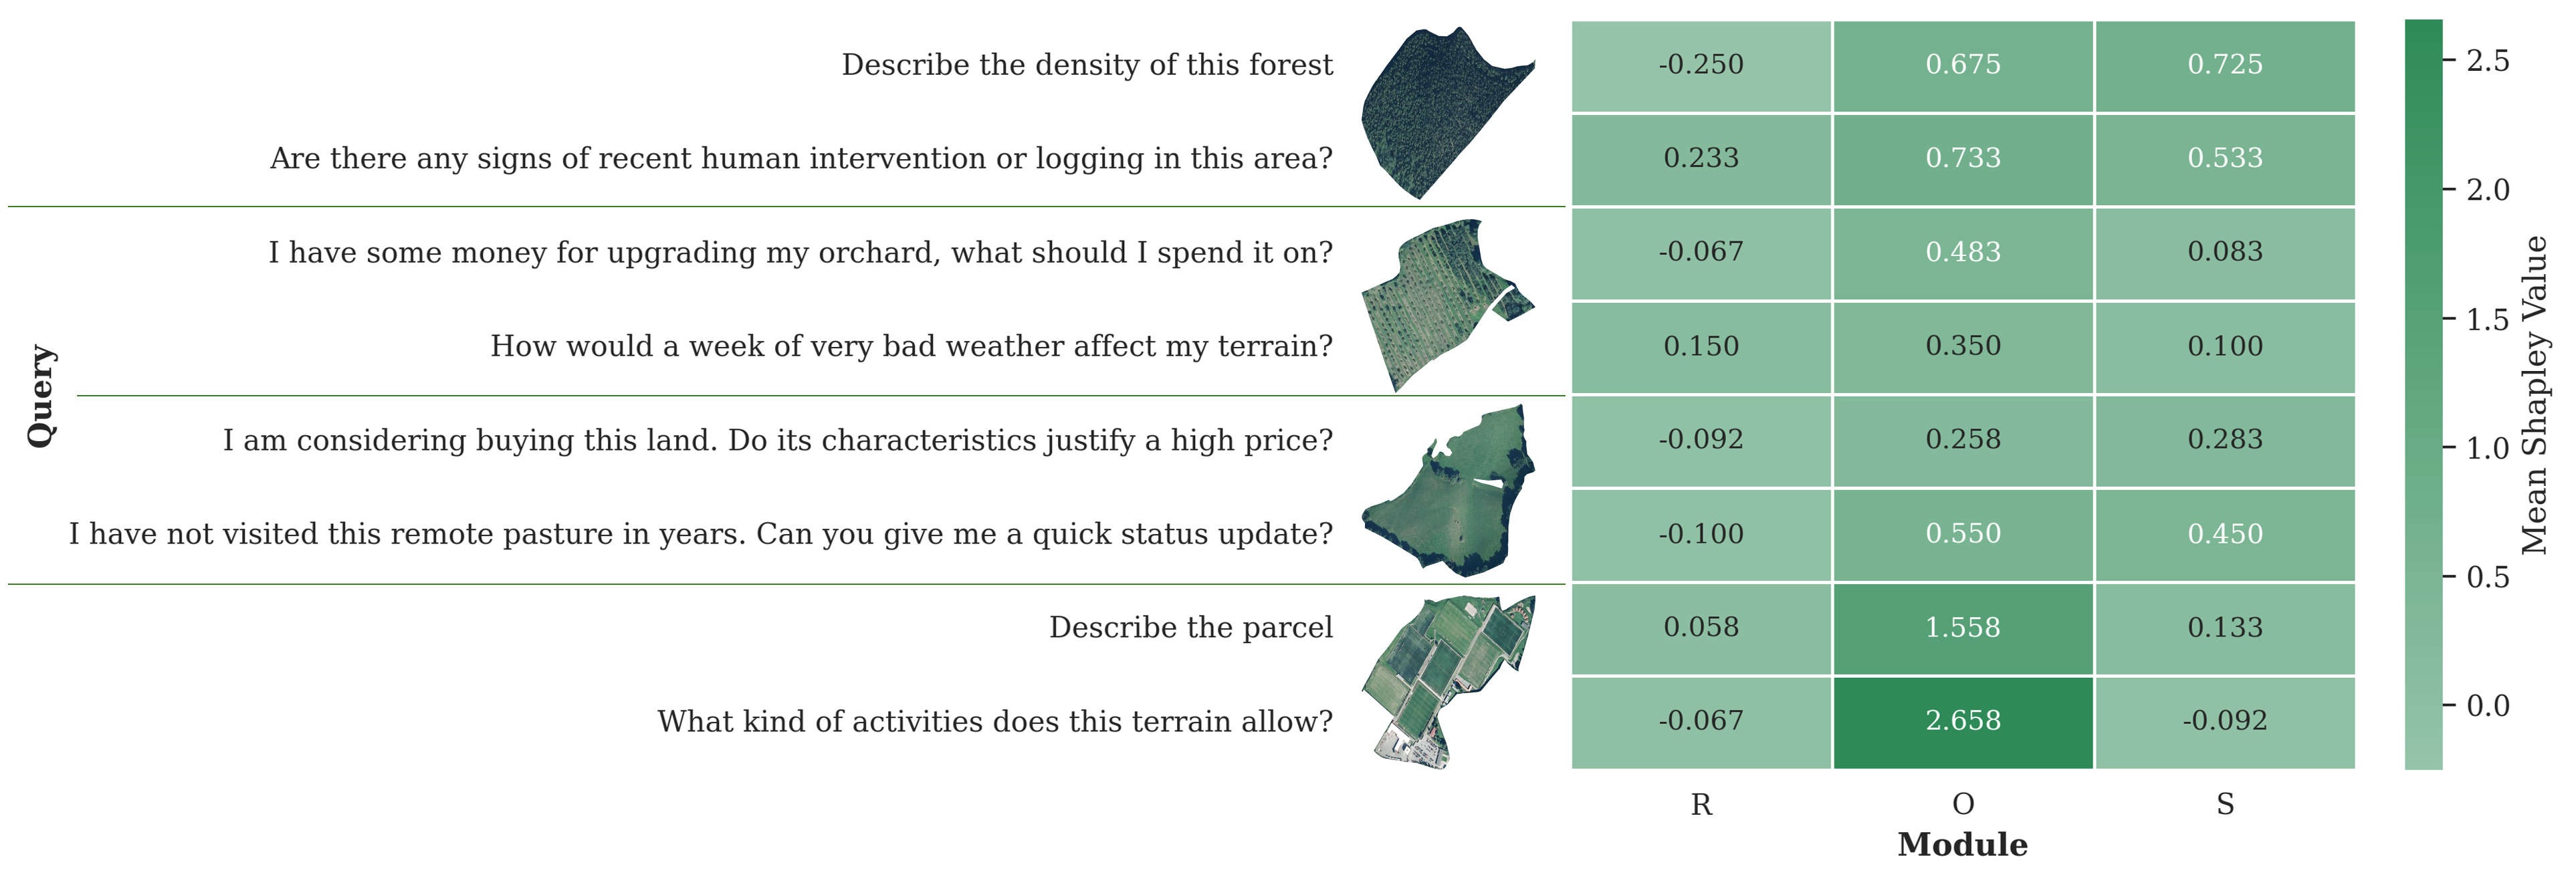
\includegraphics[width=\columnwidth]{PIC/shapleys_queries_greens.png}}
% 	\caption{}
% 	\label{fig:shapleys_queries}
% \end{figure}

\begin{figure*}[t]
	\centering{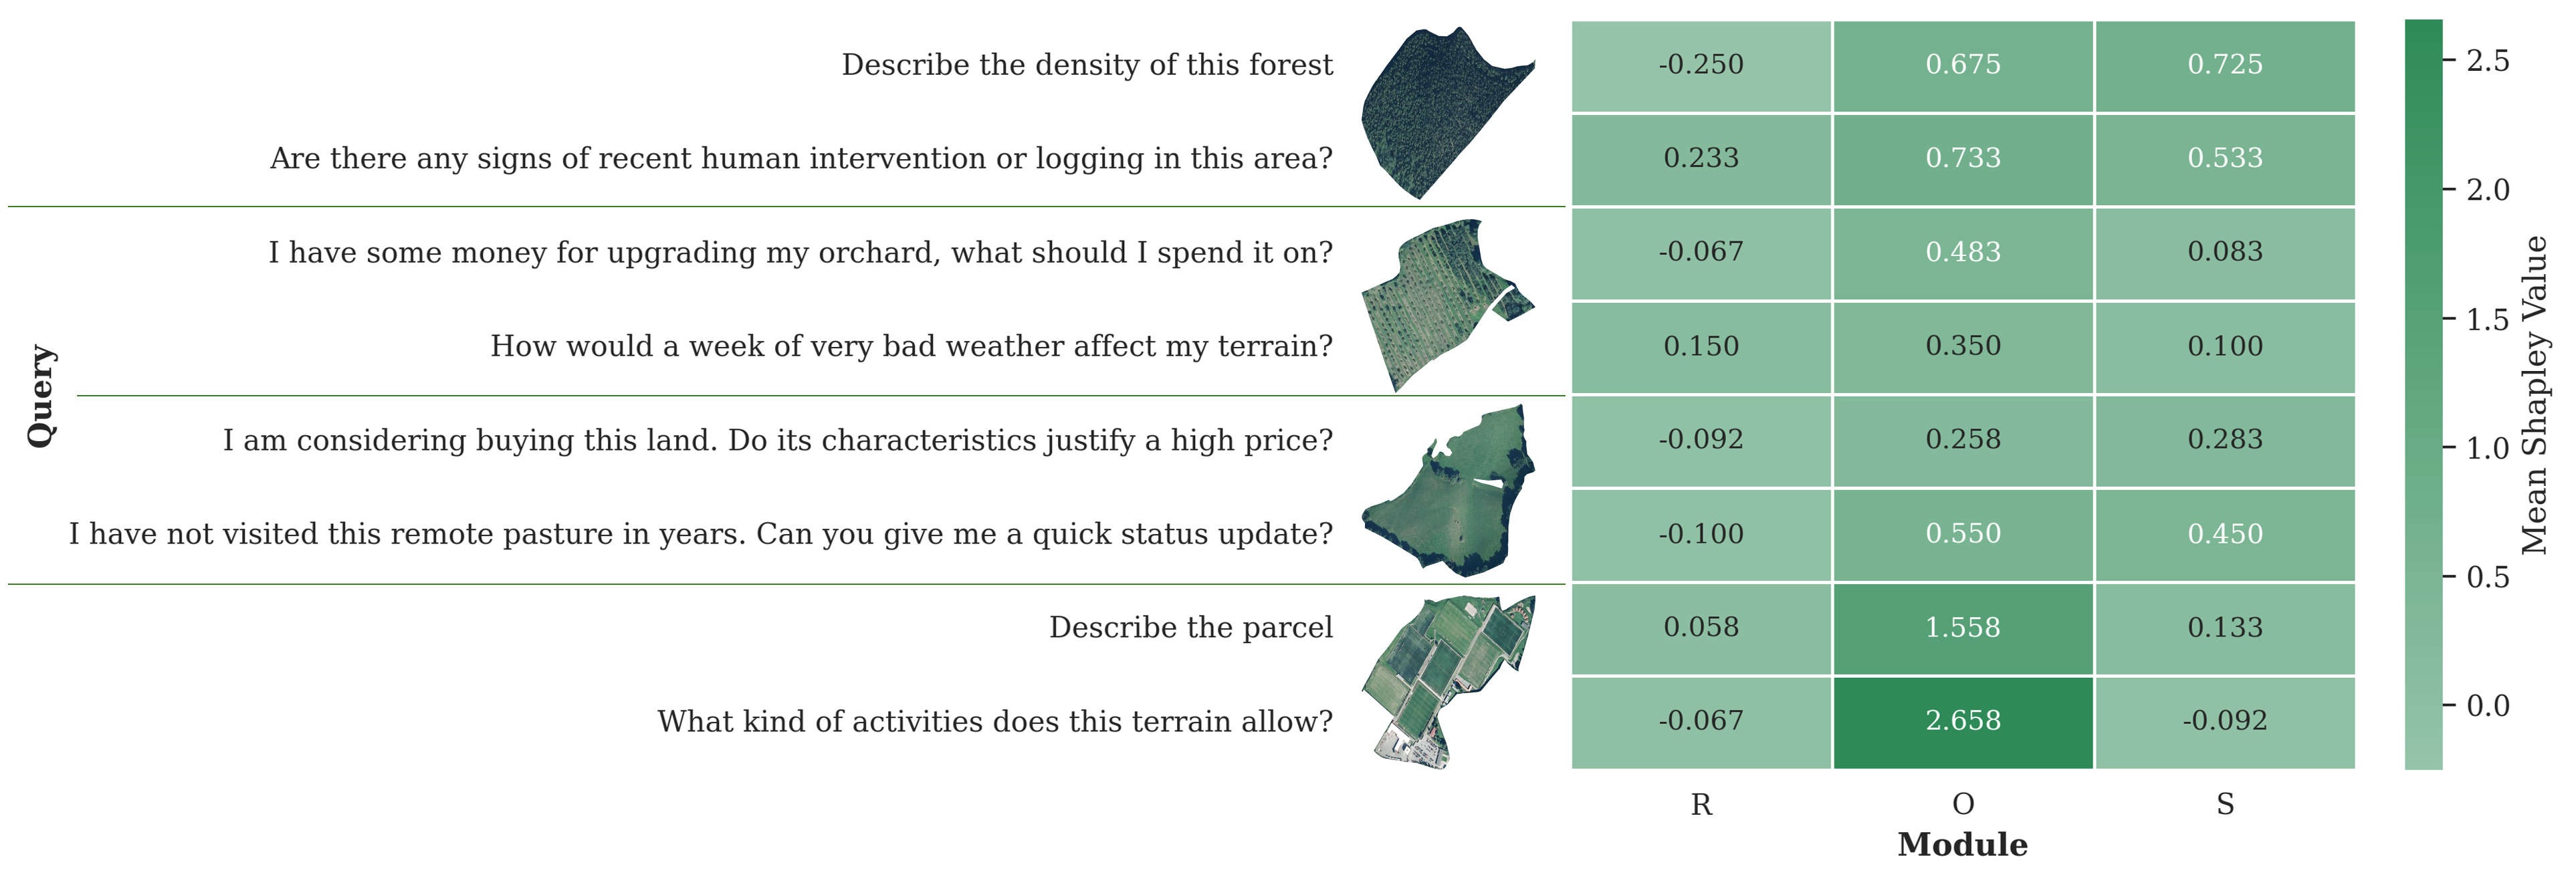
\includegraphics[width=\textwidth]{PIC/shapleys_queries_greens.png}}
	\caption{}
	\label{fig:shapleys_queries_2}
\end{figure*}





\textcolor{red}{Referencia a zenodo con dataset anonimizado}

\section{Conclusions}

\section*{Acknowledgements}
Thanks to ...

%% The Appendices part is started with the command \appendix;
%% appendix sections are then done as normal sections
\appendix

\section{Appendix A: Shapley values}
%% \label{}

\begin{table*}[htbp]
\centering
\caption{Shapley}
\label{tab:}

\renewcommand{\arraystretch}{0.9} 
\setlength{\tabcolsep}{4pt}        
\scriptsize                        

\begin{tabular}{>{\centering\arraybackslash}p{0.1\textwidth}
		>{\raggedright\arraybackslash}p{0.2\textwidth}
		p{0.1\textwidth}
		>{\centering\arraybackslash}p{0.1\textwidth}
		>{\centering\arraybackslash}p{0.2\textwidth}
		>{\centering\arraybackslash}p{0.2\textwidth}
	}
\toprule
\textbf{Judge} & \textbf{Metric} & \textbf{Module} & \textbf{Shapley Value} & \textbf{Relative Contribution (\%)} & \textbf{Global Delta} \\
\midrule
\multirow{15}{*}{H\_C} & \multirow{3}{*}{Correctness} & R & 0.167 & 16.67\% & \multirow{3}{*}{1.000} \\
 &  & O & 0.729 & 72.92\% &  \\
 &  & S & 0.104 & 10.42\% &  \\
\cmidrule(lr){2-6}
 & \multirow{3}{*}{Completeness} & R & 0.396 & 12.18\% & \multirow{3}{*}{3.250} \\
 &  & O & 2.083 & 64.10\% &  \\
 &  & S & 0.771 & 23.72\% &  \\
\cmidrule(lr){2-6}
 & \multirow{3}{*}{Relevance} & R & 0.229 & 9.65\% & \multirow{3}{*}{2.375} \\
 &  & O & 1.854 & 78.07\% &  \\
 &  & S & 0.292 & 12.28\% &  \\
\cmidrule(lr){2-6}
 & \multirow{3}{*}{Utility} & R & 0.271 & 8.67\% & \multirow{3}{*}{3.125} \\
 &  & O & 2.208 & 70.67\% &  \\
 &  & S & 0.646 & 20.67\% &  \\
\cmidrule(lr){2-6}
 & \multirow{3}{*}{Grounding} & R & 0.208 & 12.82\% & \multirow{3}{*}{1.625} \\
 &  & O & 1.208 & 74.36\% &  \\
 &  & S & 0.208 & 12.82\% &  \\
\midrule
\multirow{15}{*}{H\_E} & \multirow{3}{*}{Correctness} & R & 0.021 & 3.33\% & \multirow{3}{*}{0.625} \\
 &  & O & 0.583 & 93.33\% &  \\
 &  & S & 0.021 & 3.33\% &  \\
\cmidrule(lr){2-6}
 & \multirow{3}{*}{Completeness} & R & -0.021 & -0.98\% & \multirow{3}{*}{2.125} \\
 &  & O & 1.541 & 72.55\% &  \\
 &  & S & 0.604 & 28.43\% &  \\
\cmidrule(lr){2-6}
 & \multirow{3}{*}{Relevance} & R & -0.146 & -7.78\% & \multirow{3}{*}{1.875} \\
 &  & O & 1.479 & 78.89\% &  \\
 &  & S & 0.542 & 28.89\% &  \\
\cmidrule(lr){2-6}
 & \multirow{3}{*}{Utility} & R & -0.104 & -6.41\% & \multirow{3}{*}{1.625} \\
 &  & O & 1.333 & 82.05\% &  \\
 &  & S & 0.396 & 24.36\% &  \\
\cmidrule(lr){2-6}
 & \multirow{3}{*}{Grounding} & R & 0.042 & 33.33\% & \multirow{3}{*}{0.125} \\
 &  & O & 0.042 & 33.33\% &  \\
 &  & S & 0.042 & 33.33\% &  \\
\midrule
\multirow{15}{*}{LLM\_Q} & \multirow{3}{*}{Correctness} & R & -0.146 & -14.58\% & \multirow{3}{*}{1.000} \\
 &  & O & 0.854 & 85.42\% &  \\
 &  & S & 0.292 & 29.17\% &  \\
\cmidrule(lr){2-6}
 & \multirow{3}{*}{Completeness} & R & -0.062 & 0.00\% & \multirow{3}{*}{0.000} \\
 &  & O & 0.062 & 0.00\% &  \\
 &  & S & 0.000 & 0.00\% &  \\
\cmidrule(lr){2-6}
 & \multirow{3}{*}{Relevance} & R & -0.250 & -50.00\% & \multirow{3}{*}{0.500} \\
 &  & O & 0.625 & 125.00\% &  \\
 &  & S & 0.125 & 25.00\% &  \\
\cmidrule(lr){2-6}
 & \multirow{3}{*}{Utility} & R & -0.062 & -6.25\% & \multirow{3}{*}{1.000} \\
 &  & O & 0.812 & 81.25\% &  \\
 &  & S & 0.250 & 25.00\% &  \\
\cmidrule(lr){2-6}
 & \multirow{3}{*}{Grounding} & R & -0.479 & -383.33\% & \multirow{3}{*}{0.125} \\
 &  & O & 0.458 & 366.67\% &  \\
 &  & S & 0.146 & 116.67\% &  \\
\midrule
\multirow{15}{*}{LLM\_G} & \multirow{3}{*}{Correctness} & R & -0.083 & -9.52\% & \multirow{3}{*}{0.875} \\
 &  & O & 0.667 & 76.19\% &  \\
 &  & S & 0.292 & 33.33\% &  \\
\cmidrule(lr){2-6}
 & \multirow{3}{*}{Completeness} & R & -0.021 & -4.17\% & \multirow{3}{*}{0.500} \\
 &  & O & 0.354 & 70.83\% &  \\
 &  & S & 0.167 & 33.33\% &  \\
\cmidrule(lr){2-6}
 & \multirow{3}{*}{Relevance} & R & -0.083 & -22.22\% & \multirow{3}{*}{0.375} \\
 &  & O & 0.292 & 77.78\% &  \\
 &  & S & 0.167 & 44.44\% &  \\
\cmidrule(lr){2-6}
 & \multirow{3}{*}{Utility} & R & 0.000 & 0.00\% & \multirow{3}{*}{0.750} \\
 &  & O & 0.500 & 66.67\% &  \\
 &  & S & 0.250 & 33.33\% &  \\
\cmidrule(lr){2-6}
 & \multirow{3}{*}{Grounding} & R & -0.208 & -41.67\% & \multirow{3}{*}{0.500} \\
 &  & O & 0.479 & 95.83\% &  \\
 &  & S & 0.229 & 45.83\% &  \\
\bottomrule
\end{tabular}
\end{table*}

%% If you have bibdatabase file and want bibtex to generate the
%% bibitems, please use
%%
\bibliographystyle{elsarticle-harv}
\bibliography{bibliography}

%% else use the following coding to input the bibitems directly in the
%% TeX file.

%%\begin{thebibliography}{00}

%% \bibitem[Author(year)]{label}
%% For example:

%% \bibitem[Aladro et al.(2015)]{Aladro15} Aladro, R., Martín, S., Riquelme, D., et al. 2015, \aas, 579, A101


%%\end{thebibliography}


\end{document}

\endinput
%%
%% End of file `elsarticle-template-harv.tex'.
